\documentclass[aspectratio=169,10pt]{beamer}
\usepackage{../common/beamer_theme_bio}

\title{\textbf{Biostatistiques Appliquées \& Modélisation du Vivant}}
\subtitle{Chapitre V : Analyse en Composantes Principales (ACP) \& Profilage Multivarié}
\author{\textbf{Dr. Sarra BENMOUMOU-HOSNI (Ph.D.)}}
\institute{
  Faculté des Sciences --- Département de Biologie\\
  Master 2 : Biochimie Appliquée\\
  \textbf{Université M'Hamed Bougara de Boumerdès (UMBB)}
}
\date{Année Universitaire 2024 -- 2025}

% Intercalaire automatique de transition entre sections (Plein écran sans débordement)
\AtBeginSection[]{
  \begin{frame}[plain]
    \vspace{2mm}
    \begin{tcolorbox}[colback=BioNavy,coltext=white,boxrule=0pt,arc=2mm,left=6pt,right=6pt,top=3pt,bottom=3pt]
      \centering\bfseries\normalsize Progression Pédagogique du Chapitre V
    \end{tcolorbox}
    \vspace{1mm}
    {\small\tableofcontents[currentsection, hideothersubsections]}
  \end{frame}
}

\begin{document}

% --- Diapositive 1 : Titre ---
\begin{frame}[plain]
  \titlepage
\end{frame}

% --- Diapositive 2 : Sommaire Général ---
\begin{frame}{Plan Détaillé du Chapitre V}
  \begin{conceptbox}{1. Fondements \& Démonstration Géométrique 2D $\to$ 1D}
    \footnotesize
    \textbf{Section 1 :} L'Ère des Données Omiques \& Le Besoin de Réduction\\
    \textbf{Section 2 :} Exemple Fil Conducteur chez la Souris : La Redondance Linéaire 2D\\
    \textbf{Section 3 :} Géométrie de l'ACP : Rotation des Axes \& Réduction vers 1D
  \end{conceptbox}
  \vspace{1mm}
  \begin{biobox}{2. Algèbre, Espaces Factoriels \& Diagnostic Multivarié}
    \footnotesize
    \textbf{Section 4 :} Algèbre Matricielle : Matrice $R$, Valeurs Propres \& Éboulis de Kaiser\\
    \textbf{Section 5 :} L'Espace des Variables : Le Cercle des Corrélations, $\cos^2$ \& Contributions\\
    \textbf{Section 6 :} L'Espace des Individus : Le Plan Factoriel des Scores (Score Plot)\\
    \textbf{Section 7 :} Pièges Méthodologiques, Sélection de Biomarqueurs \& Synthèse
  \end{biobox}
\end{frame}

% ========================================================
\section{L'Ère des Données Omiques \& Le Besoin de Réduction}
% ========================================================

% --- Diapositive 3 : Défi Haute Dimensionnalité ---
\begin{frame}{Le Défi Omique : L'Explosion de la Haute Dimensionnalité}
  \begin{biobox}{La Matrice Expérimentale Moderne ($n \times p$)}
    \footnotesize
    En biochimie médicale, spectrométrie de masse, métabolomique et transcriptomique :
    \begin{itemize}
      \item $n$ échantillons biologiques (lignes : souris, patients, lysats tissulaires).
      \item $p$ biomarqueurs dosés simultanément (colonnes : métabolites, lipides, transaminases, cytokines).
      \item Un seul passage en LC-MS/MS quantifie simultanément 40 à 300 métabolites par goutte de plasma !
    \end{itemize}
  \end{biobox}
  \vspace{1mm}
  \begin{warnbox}{Pourquoi l'Approche Univariée Classique Échoue ?}
    \footnotesize
    \begin{itemize}
      \item Tester les 40 métabolites un par un (40 tests $t$ ou ANOVA séparés) multiplie le risque d'erreur globale $\alpha$ (faux positifs).
      \item Plus grave encore : cela \textbf{ignore totalement les corrélations biologiques} entre molécules appartenant à une même voie métabolique !
    \end{itemize}
  \end{warnbox}
\end{frame}

% --- Diapositive 4 : Mission Fondamentale ACP ---
\begin{frame}{La Mission Fondamentale de l'ACP : Réduction Non Supervisée}
  \begin{conceptbox}{Définition Statistique : Comprimer Sans Perdre l'Essentiel}
    \footnotesize
    L'\textbf{Analyse en Composantes Principales (ACP)} est une méthode de réduction de dimensionnalité qui transforme $p$ variables de départ corrélées en un petit nombre $k$ ($k \ll p$, typiquement 2 ou 3) de nouvelles variables \textbf{artificielles, non corrélées entre elles} appelées \textbf{composantes principales} :
    \begin{equation*}
      \mathbb{R}^p \xrightarrow{\quad \text{Projection orthogonale} \quad} \mathbb{R}^k \quad (k = 2 \text{ ou } 3)
    \end{equation*}
  \end{conceptbox}
  \vspace{1mm}
  \begin{takeawaybox}{Les Trois Objectifs Majeurs pour le Biochimiste}
    \footnotesize
    \begin{enumerate}
      \item \textbf{Résumer :} Conserver le maximum de l'inertie (variance biologique totale) sur un plan 2D lisible à l'œil nu.
      \item \textbf{Détecter la redondance :} Identifier les groupes de biomarqueurs qui évoluent de concert (voies métaboliques).
      \item \textbf{Discriminer :} Séparer spontanément les états phénotypiques (Sains vs Pathologiques) de manière non supervisée.
    \end{enumerate}
  \end{takeawaybox}
\end{frame}

% ========================================================
\section{Exemple Fil Conducteur chez la Souris : La Redondance Linéaire 2D}
% ========================================================

% --- Diapositive 5 : Protocole Préclinique Souris ---
\begin{frame}{Étude Préclinique chez la Souris : Modèle d'Obésité Métabolique}
  \begin{biobox}{Protocole Expérimental ($N = 24$ Souris C57BL/6J)}
    \footnotesize
    Pour comprendre la mécanique géométrique de l'ACP, étudions un modèle préclinique concret d'adiposité :
    \begin{itemize}
      \item \textbf{Groupe 1 (Témoins Chow, $n = 12$) :} Souris nourries avec une alimentation standard de laboratoire.
      \item \textbf{Groupe 2 (Obèses HFD, $n = 12$) :} Souris soumises à un régime riche en lipides (\textit{High-Fat Diet}, 60\% kcal de graisse).
    \end{itemize}
    On mesure sur chaque souris deux variables biométriques classiques :
    \begin{enumerate}
      \item \textbf{Variable 1 ($X_1$) :} Poids corporel total (exprimé en grammes, g).
      \item \textbf{Variable 2 ($X_2$) :} Masse du tissu adipeux épididymaire (exprimée en milligrammes, mg).
    \end{enumerate}
  \end{biobox}
  \vspace{1mm}
  \begin{conceptbox}{La Question Pédagogique Fondamentale}
    \footnotesize
    Puisque le tissu adipeux augmente directement avec le poids total, les deux variables sont fortement liées.\\
    \textbf{Comment l'ACP peut-elle réduire ces 2 variables dépendantes en 1 seul axe synthétique d'adiposité sans perte d'information ?}
  \end{conceptbox}
\end{frame}

% --- Diapositive 6 : Notion 1 : Redondance Lineaire 2D ---
\begin{frame}{Notion 1 : Le Constat Biologique de Redondance Linéaire}
  \begin{conceptbox}{Corrélation Linéaire Élevée : L'Effet « Cigare »}
    \footnotesize
    Lorsque deux variables mesurent deux facettes d'un même phénomène physiologique, les points expérimentaux s'étirent le long d'une diagonale dans l'espace 2D :
    \begin{equation*}
      r(X_1, X_2) = \frac{\sum (X_{i1} - \bar{X}_1)(X_{i2} - \bar{X}_2)}{\sqrt{SS_{X_1} \cdot SS_{X_2}}} = \mathbf{+0.96} \quad (p < 10^{-10})
    \end{equation*}
  \end{conceptbox}
  \vspace{1mm}
  \begin{biobox}{Le Diagnostic du Biochimiste : Pourquoi Conserver Deux Axes ?}
    \footnotesize
    \begin{itemize}
      \item Si l'on connaît le poids corporel d'une souris ($45\,\text{g}$), on peut prédire avec une excellente précision sa masse adipeuse ($1450\,\text{mg}$).
      \item Les deux axes $X_1$ et $X_2$ portent à $96\%$ la \textbf{même information biologique}.
      \item Un espace à 2 dimensions est redondant : un seul axe incliné suffirait à décrire l'essentiel de la variabilité entre souris !
    \end{itemize}
  \end{biobox}
\end{frame}

% --- Diapositive 7 : Visualisation 2D Redondance ---
\begin{frame}{Visualisation Graphique : La Redondance Linéaire 2D chez la Souris}
  \begin{center}
    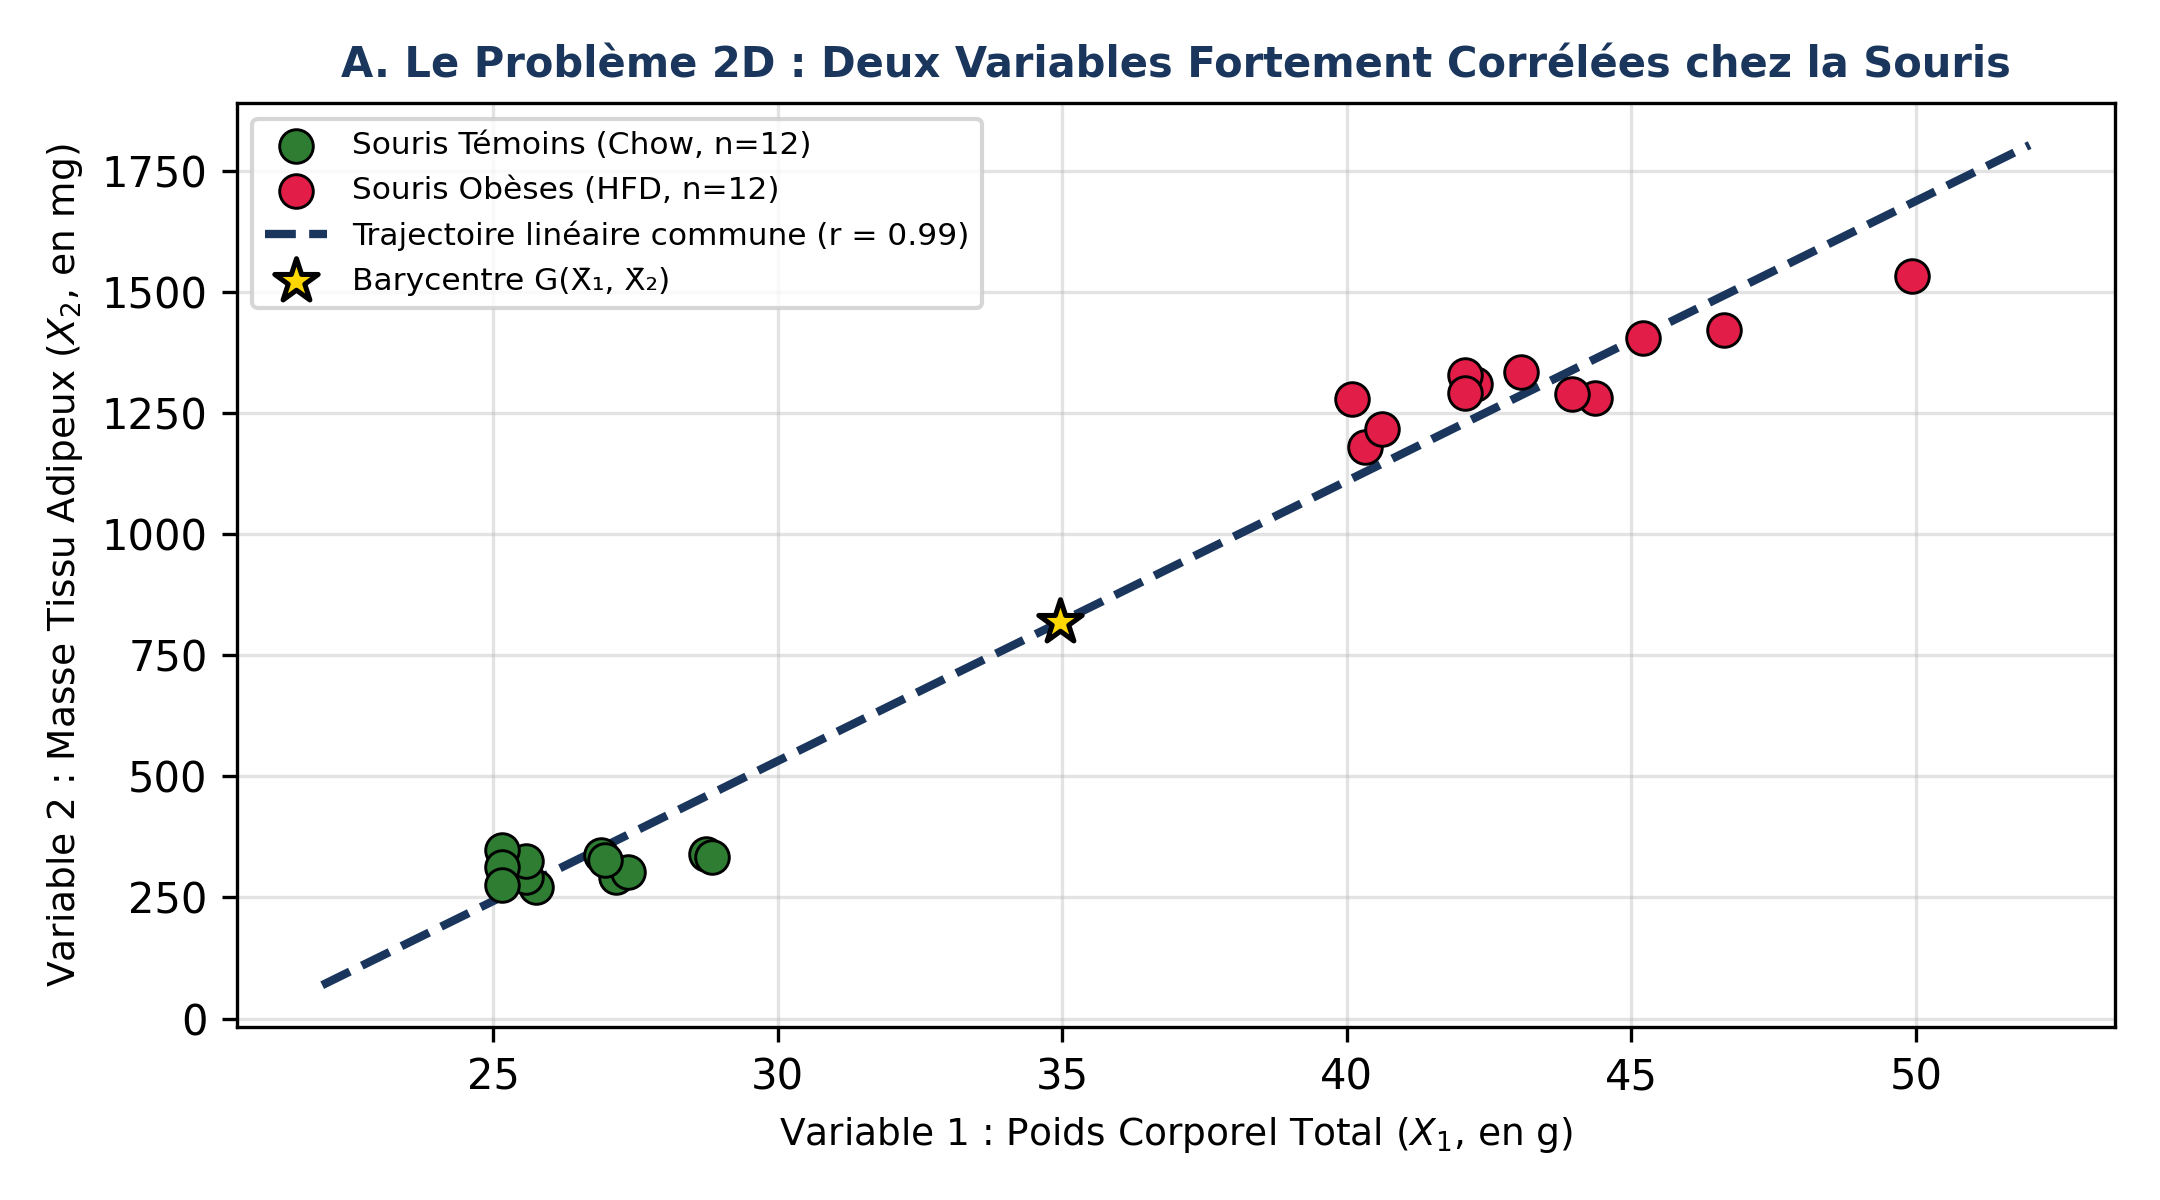
\includegraphics[height=0.55\textheight]{../figures/fig05_mice_2d_redundancy.png}
  \end{center}
  \vspace{-1mm}
  \begin{takeawaybox}{Lecture du Graphique 2D}
    \scriptsize
    Les souris témoins (vert) et obèses (rouge) s'alignent sur une trajectoire linéaire unique ($r = 0.96$). La variabilité perpendiculaire à cette droite est minime (simple bruit biologique individuel).
  \end{takeawaybox}
\end{frame}

% --- Diapositive 8 : Notion 2 : Centrage-Reduction ---
\begin{frame}{Notion 2 : Pourquoi l'Étape de Centrage-Réduction est Impérative ?}
  \begin{warnbox}{Le Piège Mortel des Échelles \& Unités Disparates}
    \footnotesize
    Comparons les dispersions numériques de nos deux grandeurs non standardisées :
    \begin{itemize}
      \item $X_1$ (Poids en g) : moyenne $\bar{X}_1 = 35.0\,\text{g}$, variance $s_1^2 \approx \mathbf{85.0\,\text{g}^2}$.
      \item $X_2$ (Adipeux en mg) : moyenne $\bar{X}_2 = 860.0\,\text{mg}$, variance $s_2^2 \approx \mathbf{280\,000\,\text{mg}^2}$ !
    \end{itemize}
    Si l'on injectait les données brutes dans l'ACP : la variable $X_2$ posséderait à elle seule $99.97\%$ de la variance numérique par le simple fait d'être mesurée en milligrammes !
  \end{warnbox}
  \vspace{1mm}
  \begin{takeawaybox}{Règle d'Or de l'ACP en Sciences de la Vie}
    \footnotesize
    En biologie, on utilise \textbf{exclusivement l'ACP normée} (centrée-réduite) basée sur la \textbf{matrice des corrélations} $R$. Chaque variable reçoit une variance initiale normalisée égale à 1, lui conférant un poids analytique équitable.
  \end{takeawaybox}
\end{frame}

% --- Diapositive 9 : Notion 3 : Transformation Z-Scores ---
\begin{frame}{Notion 3 : La Transformation en Variables Centrées-Réduites ($Z$)}
  \begin{conceptbox}{Formule Mathématique du $Z$-Score}
    \footnotesize
    Chaque mesure individuelle $X_{ij}$ (souris $i$, variable $j$) est transformée selon :
    \begin{equation*}
      Z_{ij} = \frac{X_{ij} - \bar{X}_j}{s_j} \quad \text{avec } \bar{X}_j = \text{moyenne de la variable } j, \quad s_j = \text{écart-type de la variable } j
    \end{equation*}
  \end{conceptbox}
  \vspace{1mm}
  \begin{biobox}{Propriétés Algébriques \& Sens Biologique}
    \footnotesize
    \begin{itemize}
      \item \textbf{Moyenne nulle :} $\mathbb{E}(Z_j) = 0 \implies$ Le nuage de points est translaté pour avoir son barycentre à l'origine $(0,0)$.
      \item \textbf{Variance unitaire :} $\text{Var}(Z_j) = 1 \implies$ Toutes les variables jouent à armes égales, sans effet d'échelle d'appareil.
      \item \textbf{Interprétation :} Une souris avec $Z_{i1} = +2.0$ a un poids corporel situé à $+2$ écarts-types au-dessus de la moyenne.
    \end{itemize}
  \end{biobox}
\end{frame}

% ========================================================
\section{Géométrie de l'ACP : Rotation des Axes \& Réduction vers 1D}
% ========================================================

% --- Diapositive 10 : Notion 4 : Principe Rotation ---
\begin{frame}{Notion 4 : Le Principe Géométrique : Rechercher la Variance Maximale}
  \begin{conceptbox}{Recherche de la Meilleure Droite de Projection}
    \footnotesize
    Au lieu de projeter sur les anciens axes $Z_1$ et $Z_2$, l'ACP fait pivoter le système de coordonnées d'un angle $\theta$ optimal :
    \begin{equation*}
      \text{Axe PC1} = \text{Direction qui rend maximale la dispersion (variance) des points projetés}
    \end{equation*}
    \textbf{Équivalence géométrique de Pythagore :}
    Maximiser la variance des projections orthogonales revient rigoureusement à \textbf{minimiser la somme des carrés des distances résiduelles} (perte d'information minimale).
  \end{conceptbox}
  \vspace{1mm}
  \begin{biobox}{Application au Modèle Souris}
    \footnotesize
    La direction de plus grand allongement de l'ellipse coïncide avec la droite passant par le centre des témoins (minces) et le centre des obèses (lourds). C'est précisément l'axe de la première composante principale (PC1).
  \end{biobox}
\end{frame}

% --- Diapositive 11 : Notion 5 : Axe PC1 ---
\begin{frame}{Notion 5 : La Première Composante Principale (PC1)}
  \begin{conceptbox}{Définition Algébrique : Combinaison Linéaire Optimale}
    \footnotesize
    La coordonnée (score) de chaque souris sur le nouvel axe PC1 est une somme pondérée des variables centrées-réduites :
    \begin{equation*}
      \text{PC1}_i = a_{11} Z_{i1} + a_{12} Z_{i2} \quad \text{avec la contrainte de normalité : } a_{11}^2 + a_{12}^2 = 1
    \end{equation*}
    Les coefficients $(a_{11}, a_{12})$ forment le premier \textbf{vecteur propre normé} $\mathbf{v}_1$.
  \end{conceptbox}
  \vspace{1mm}
  \begin{biobox}{Vecteur Propre Obtenu chez la Souris}
    \footnotesize
    Pour notre jeu de données à forte corrélation ($r = 0.96$) :
    \begin{equation*}
      \mathbf{v}_1 = \begin{pmatrix} 0.707 \\ 0.707 \end{pmatrix} \implies \mathbf{\text{PC1}_i = 0.707 \cdot Z_{i1} + 0.707 \cdot Z_{i2}}
    \end{equation*}
    \textbf{Sens biologique :}
    Les deux variables contribuent de façon exactement égale et positive à l'axe PC1. Plus une souris est lourde et adipeuse, plus son score PC1 est fortement positif !
  \end{biobox}
\end{frame}

% --- Diapositive 12 : Notion 6 : Axe PC2 Orthogonal ---
\begin{frame}{Notion 6 : La Deuxième Composante Principale (PC2) : L'Orthogonalité}
  \begin{conceptbox}{Définition de l'Axe Orthogonal (Non Corrélé)}
    \footnotesize
    Le deuxième axe PC2 doit être \textbf{strictement perpendiculaire} à PC1 ($\mathbf{v}_1 \cdot \mathbf{v}_2 = 0$) tout en captant le maximum de la variance résiduelle :
    \begin{equation*}
      \mathbf{v}_2 = \begin{pmatrix} -0.707 \\ +0.707 \end{pmatrix} \implies \mathbf{\text{PC2}_i = -0.707 \cdot Z_{i1} + 0.707 \cdot Z_{i2}}
    \end{equation*}
    \textbf{Propriété statistique fondamentale :} $\text{cor}(\text{PC1}, \text{PC2}) = 0$. Les deux axes sont mathématiquement indépendants !
  \end{conceptbox}
  \vspace{1mm}
  \begin{biobox}{Interprétation Biologique du Contraste sur PC2}
    \footnotesize
    \begin{itemize}
      \item $\text{PC2}$ oppose la masse adipeuse au poids corporel (différence $Z_{i2} - Z_{i1}$).
      \item Une souris avec un score $\text{PC2} > 0$ possède un tissu adipeux disproportionné par rapport à sa corpulence générale.
      \item Une souris avec $\text{PC2} < 0$ est plus musclée ou dense (poids élevé mais adipeux modéré).
    \end{itemize}
  \end{biobox}
\end{frame}

% --- Diapositive 13 : Visualisation Rotation Axes ---
\begin{frame}{Visualisation Graphique : La Rotation des Axes chez la Souris}
  \begin{center}
    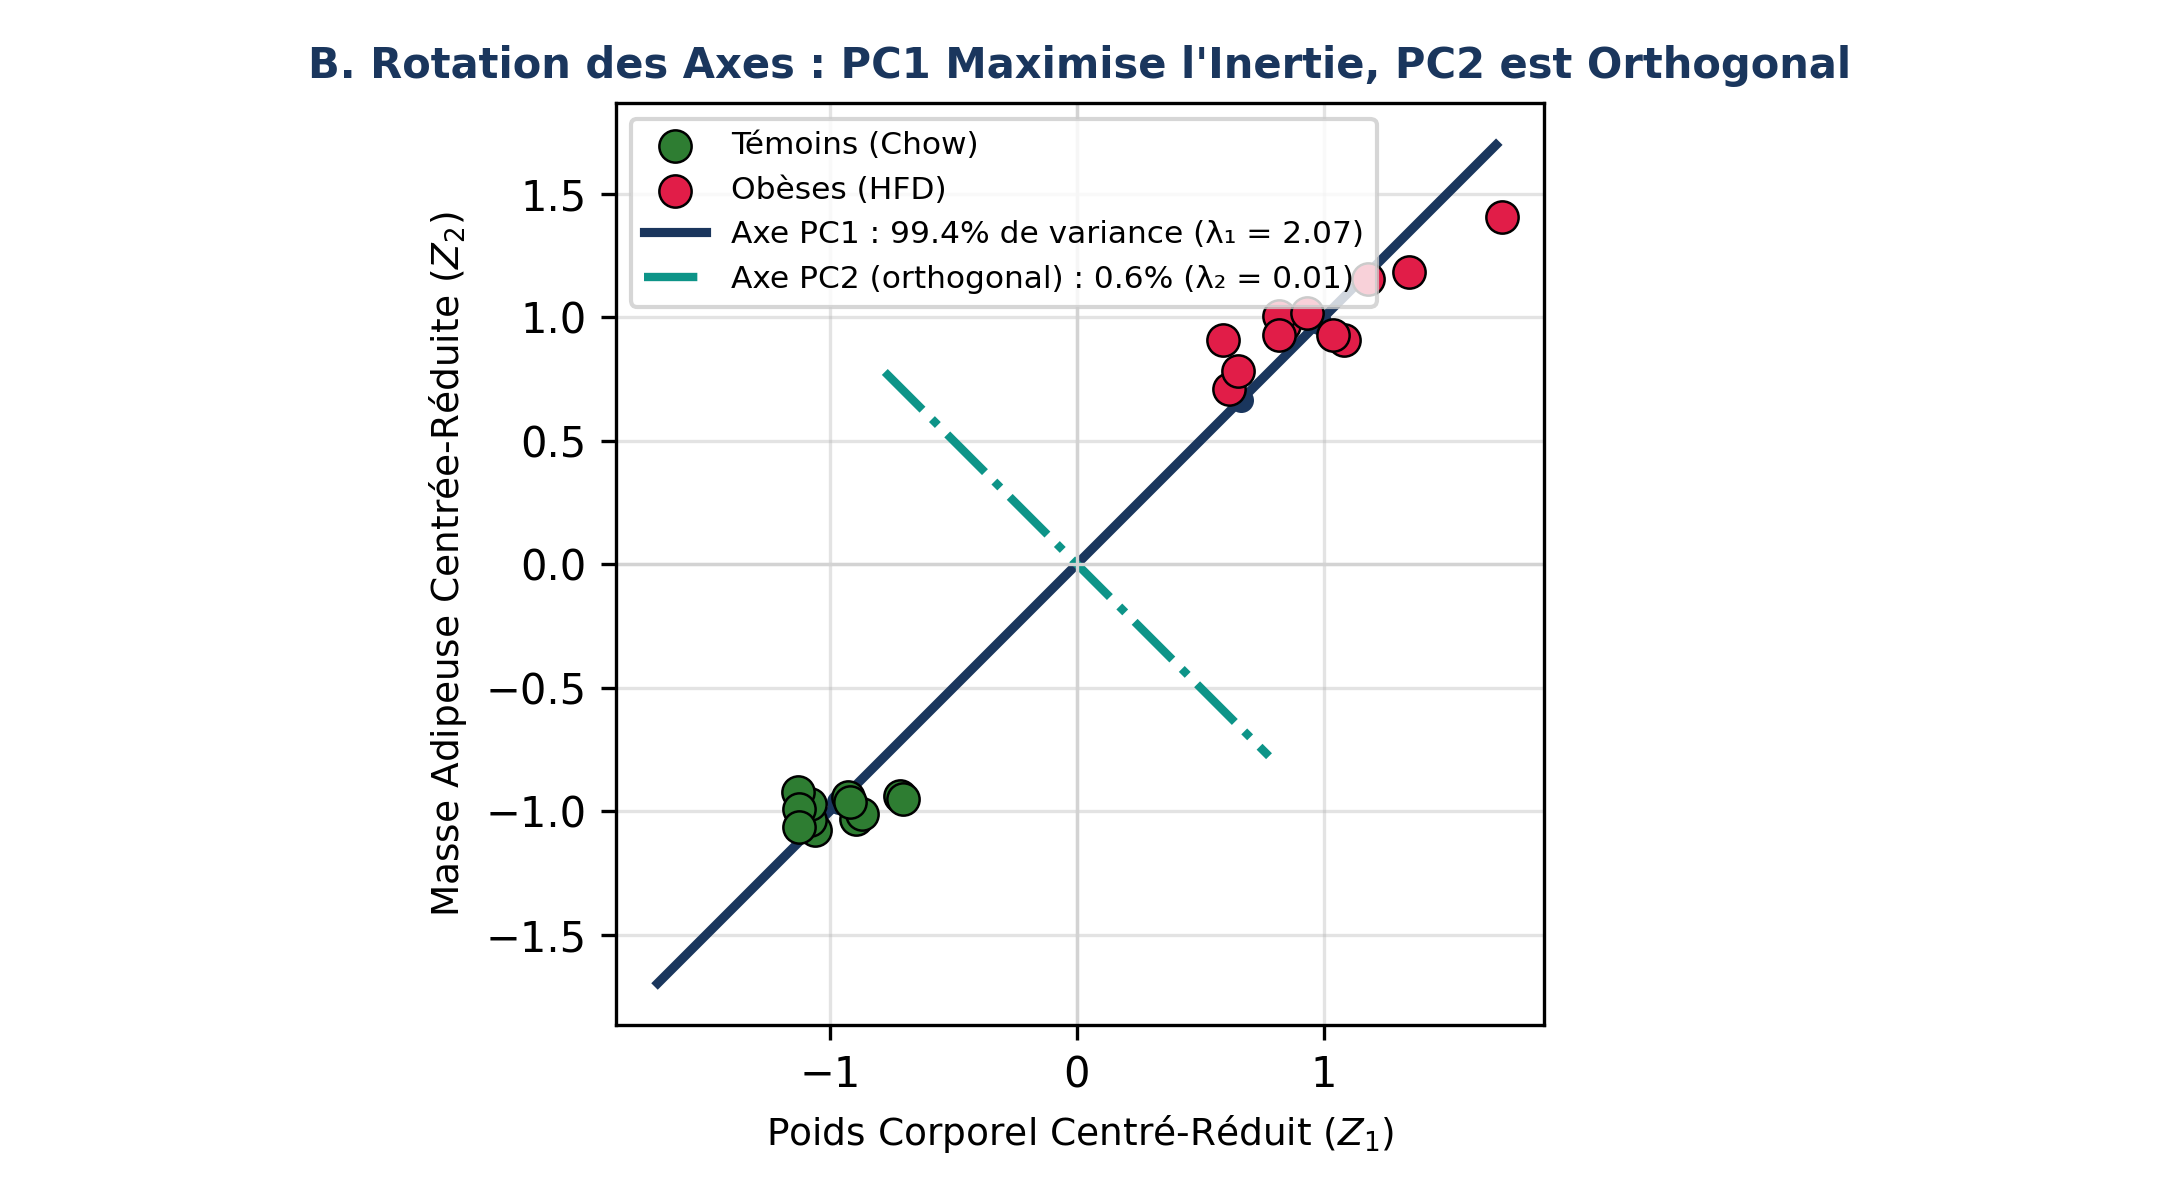
\includegraphics[height=0.55\textheight]{../figures/fig05_mice_pca_axes_rotation.png}
  \end{center}
  \vspace{-1mm}
  \begin{takeawaybox}{Lecture Géométrique}
    \scriptsize
    L'axe PC1 (bleu foncé) s'aligne sur le grand axe de l'ellipse de dispersion. L'axe PC2 (turquoise) est orthogonal. Les traits pointillés illustrent la projection orthogonale sans déformation de chaque souris sur PC1.
  \end{takeawaybox}
\end{frame}

% --- Diapositive 14 : Notion 7 : Reduction 2D vers 1D ---
\begin{frame}{Notion 7 : Comment l'ACP Réduit 2 Dimensions Corréles en 1 Seule ?}
  \begin{conceptbox}{Bilan de Variance : Partition de l'Inertie Totale}
    \footnotesize
    \begin{itemize}
      \item \textbf{Inertie totale de départ :} $\text{Var}(Z_1) + \text{Var}(Z_2) = 1.0 + 1.0 = \mathbf{2.00}$ (Inertie totale = $p$).
      \item \textbf{Variance captée par PC1 :} $\lambda_1 = \mathbf{1.93}$ (soit $\frac{1.93}{2.00} \times 100 = \mathbf{96.5\%}$ de toute l'information !).
      \item \textbf{Variance résiduelle sur PC2 :} $\lambda_2 = \mathbf{0.07}$ (soit $\frac{0.07}{2.00} \times 100 = \mathbf{3.5\%}$).
    \end{itemize}
  \end{conceptbox}
  \vspace{1mm}
  \begin{takeawaybox}{La Décision de Réduction : Abandonner PC2}
    \footnotesize
    En abandonnant purement et simplement l'axe PC2, le biologiste :
    \begin{enumerate}
      \item Ne perd que $3.5\%$ d'aléa ou de bruit individuel mineur.
      \item \textbf{Conserve $96.5\%$ de la variabilité biologique réelle} dans une seule dimension composite (PC1).
      \item Réduit un tableau 2D complexe en une échelle 1D continue et intuitive.
    \end{enumerate}
  \end{takeawaybox}
\end{frame}

% --- Diapositive 15 : Visualisation 1D Reduction ---
\begin{frame}{Visualisation Graphique : Les Souris Projetées sur l'Axe Unique PC1}
  \begin{center}
    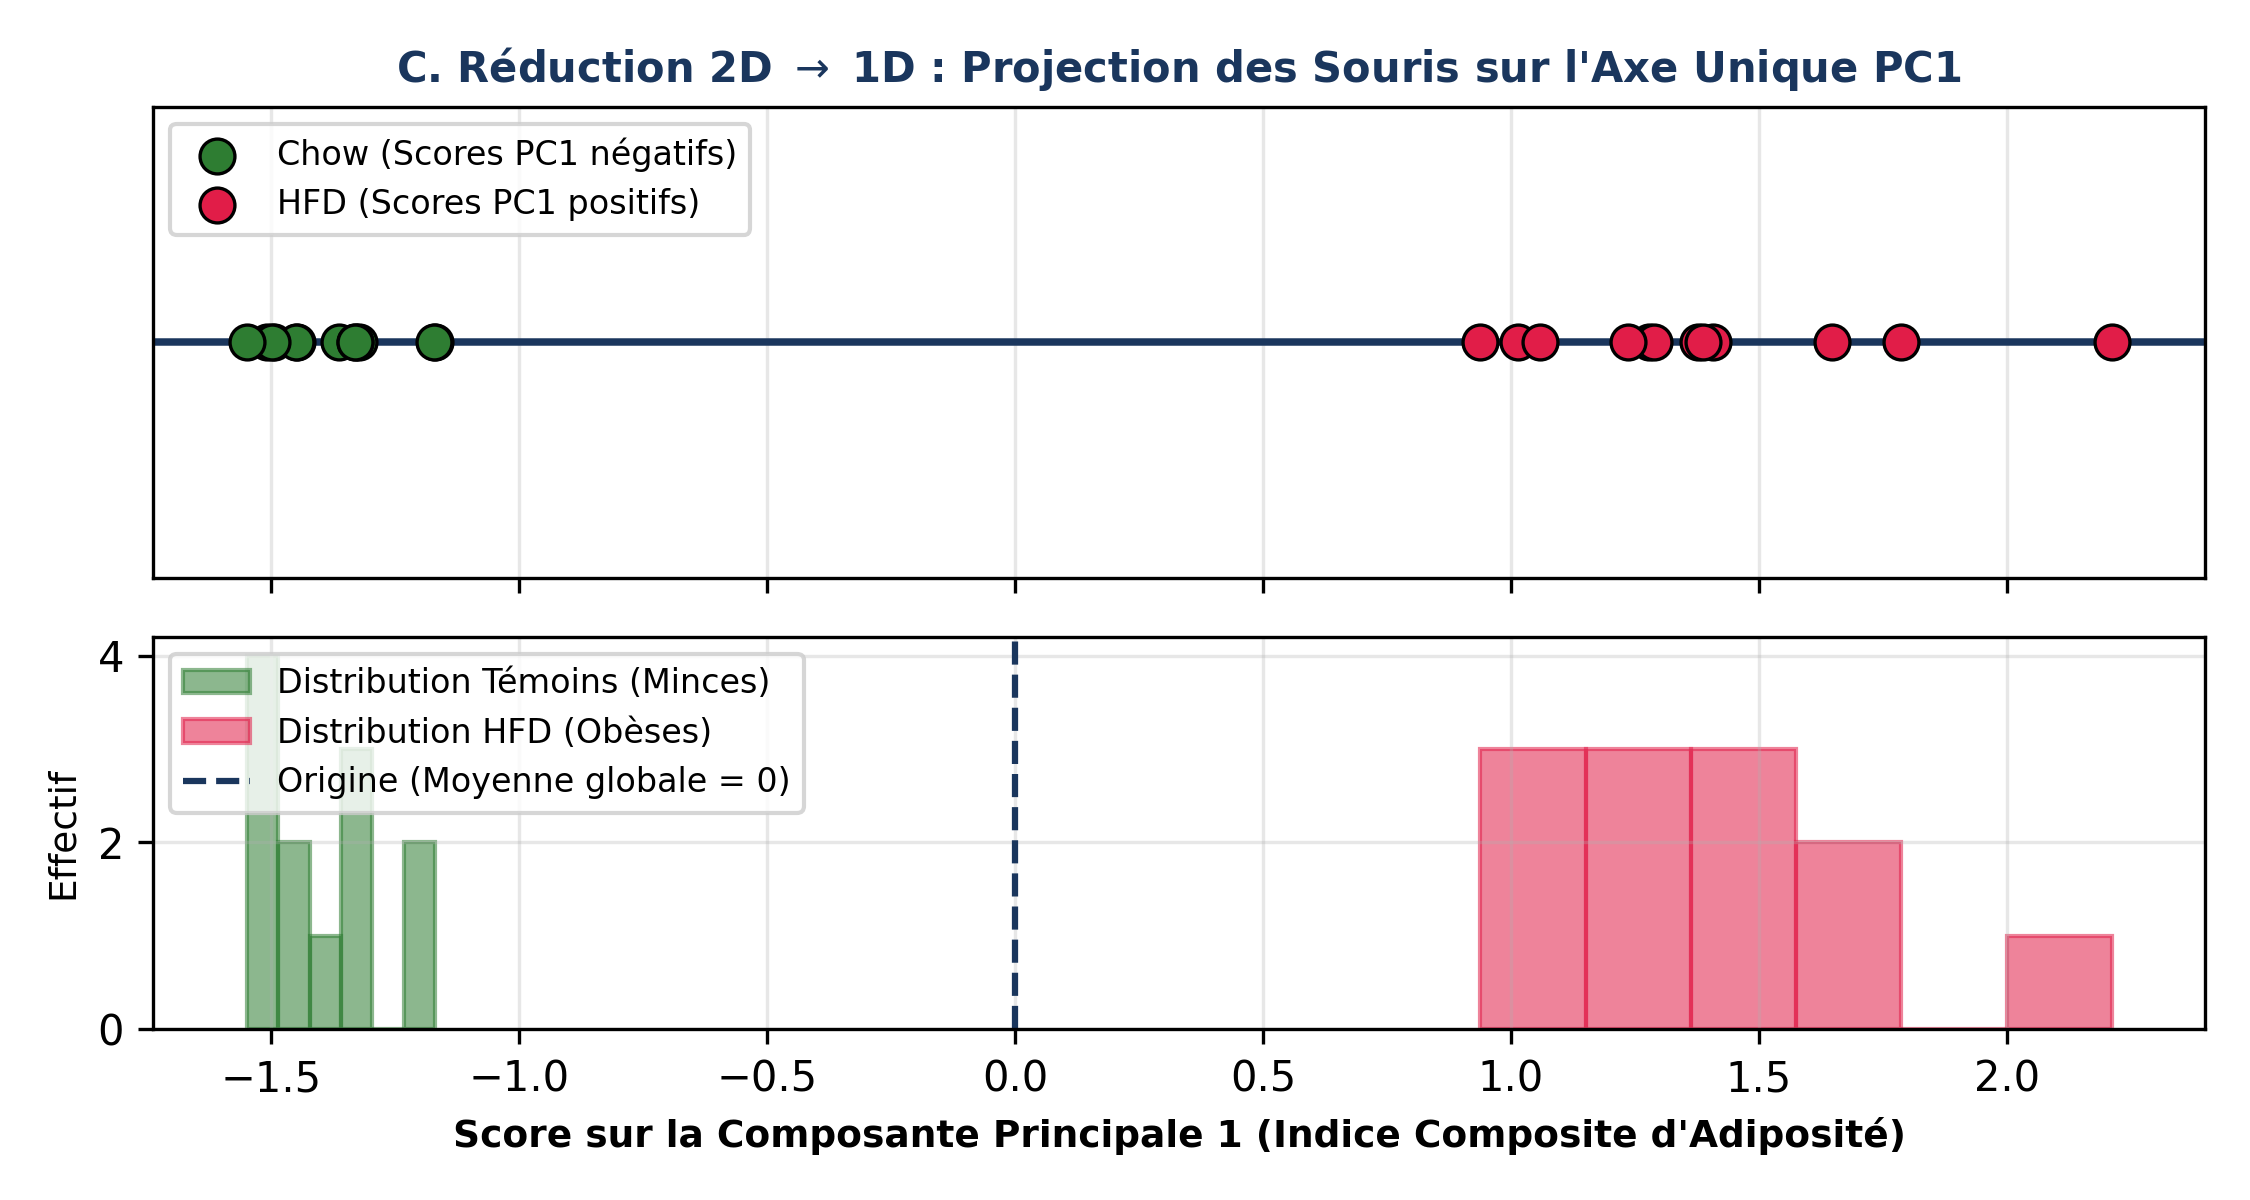
\includegraphics[height=0.55\textheight]{../figures/fig05_mice_1d_reduction.png}
  \end{center}
  \vspace{-1mm}
  \begin{takeawaybox}{Séparation Phénotypique en 1D}
    \scriptsize
    Sur l'axe 1D unique PC1, la frontière entre souris témoins (vert) et souris obèses (rouge) est absolue ($p < 10^{-8}$). La distribution montre une séparation bimodale parfaite.
  \end{takeawaybox}
\end{frame}

% --- Diapositive 16 : Notion 8 : Sens Biologique Score 1D ---
\begin{frame}{Notion 8 : Sens Biologique du Nouveau Score 1D}
  \begin{conceptbox}{L'Émergence d'une Variable Synthétique Latente}
    \footnotesize
    L'axe PC1 n'est plus ni la variable « Poids » ni la variable « Tissu Adipeux » :\\
    Il s'agit d'un \textbf{Score Composite d'Adiposité Globale / Sévérité Métabolique}.
  \end{conceptbox}
  \vspace{1mm}
  \begin{biobox}{Application Biomédicale \& Pharmacologique}
    \footnotesize
    \begin{itemize}
      \item \textbf{Souris Témoins (Chow) :} Scores PC1 négatifs ($\text{PC1} \in [-2.5 \,;\, -0.5]$). Phénotype mince et métaboliquement sain.
      \item \textbf{Souris HFD (Régime gras) :} Scores PC1 positifs ($\text{PC1} \in [+0.5 \,;\, +2.8]$). Phénotype obèse pathologique.
      \item \textbf{Évaluation d'un traitement antidiabétique :} Si une molécule thérapeutique ramène les scores PC1 des souris HFD de $+2.2$ à $-0.4$, son efficacité globale est démontrée sur un indice synthétique validé sans redondance !
    \end{itemize}
  \end{biobox}
\end{frame}

% ========================================================
\section{Algèbre Matricielle : Matrice R, Valeurs Propres \& Kaiser}
% ========================================================

% --- Diapositive 17 : Notion 9 : Matrice R ---
\begin{frame}{Notion 9 : La Matrice des Corrélations $R$ ($p \times p$)}
  \begin{conceptbox}{Structure Mathématique de la Matrice $R$}
    \footnotesize
    Pour $p$ variables biologiques centrées-réduites, la matrice de corrélation s'écrit :
    \begin{equation*}
      R = \frac{1}{n} Z^T Z = \begin{pmatrix} 1 & r_{12} & \cdots & r_{1p} \\ r_{21} & 1 & \cdots & r_{2p} \\ \vdots & \vdots & \ddots & \vdots \\ r_{p1} & r_{p2} & \cdots & 1 \end{pmatrix} \quad \text{Dans notre exemple 2D : } R = \begin{pmatrix} 1.00 & 0.96 \\ 0.96 & 1.00 \end{pmatrix}
    \end{equation*}
  \end{conceptbox}
  \vspace{1mm}
  \begin{biobox}{Propriétés Capitales pour l'ACP}
    \footnotesize
    \begin{itemize}
      \item $R$ est une matrice \textbf{carrée symétrique} ($r_{jk} = r_{kj}$) semi-définie positive.
      \item Sa diagonale principale est constituée exclusivement de 1 (corrélation de chaque variable avec elle-même).
      \item C'est cette matrice $R$ qui est diagonalisée pour extraire les axes de variabilité biologique.
    \end{itemize}
  \end{biobox}
\end{frame}

% --- Diapositive 18 : Notion 10 : Equation Valeurs Propres ---
\begin{frame}{Notion 10 : L'Équation aux Valeurs Propres : $R \mathbf{v} = \lambda \mathbf{v}$}
  \begin{conceptbox}{Théorie Spectrale de Diagonalisation}
    \footnotesize
    La recherche des axes principaux équivaut à trouver les scalaires $\lambda$ et les vecteurs $\mathbf{v} \neq 0$ vérifiant :
    \begin{equation*}
      R \mathbf{v} = \lambda \mathbf{v} \iff (R - \lambda I) \mathbf{v} = 0 \implies \det(R - \lambda I) = 0
    \end{equation*}
  \end{conceptbox}
  \vspace{1mm}
  \begin{biobox}{Résolution Analytique Complète sur l'Exemple Souris ($p = 2$)}
    \footnotesize
    \begin{equation*}
      \det \begin{pmatrix} 1 - \lambda & 0.96 \\ 0.96 & 1 - \lambda \end{pmatrix} = (1 - \lambda)^2 - 0.96^2 = 0 \implies (1 - \lambda) = \pm 0.96
    \end{equation*}
    \begin{equation*}
      \mathbf{\lambda_1 = 1 + 0.96 = 1.96}, \qquad \mathbf{\lambda_2 = 1 - 0.96 = 0.04}
    \end{equation*}
    $\implies$ La première valeur propre capte $1.96$ sur une inertie totale de $2$, soit $\mathbf{98.0\%}$ de l'information théorique !
  \end{biobox}
\end{frame}

% --- Diapositive 19 : Notion 11 : Trace de R et Inertie ---
\begin{frame}{Notion 11 : La Trace de la Matrice \& Conservation de l'Inertie Totale}
  \begin{conceptbox}{Théorème Fondamental de Conservation de l'Inertie}
    \footnotesize
    La somme de toutes les valeurs propres $\lambda_k$ est rigoureusement égale à la \textbf{trace} de la matrice $R$ :
    \begin{equation*}
      \mathbf{\sum_{k=1}^p \lambda_k = \text{Tr}(R) = p} \quad \text{(Le nombre total de variables de départ)}
    \end{equation*}
  \end{conceptbox}
  \vspace{1mm}
  \begin{takeawaybox}{Principe Fondamental de Conservation}
    \footnotesize
    \begin{itemize}
      \item L'ACP ne génère aucune information nouvelle et n'en détruit aucune lors de la diagonalisation.
      \item L'inertie totale de départ ($p$) est simplement \textbf{redistribuée de façon décroissante} :
      \begin{equation*}
        \lambda_1 \ge \lambda_2 \ge \dots \ge \lambda_p \ge 0
      \end{equation*}
      \item Les premiers axes concentrent la quasi-totalité du signal utile, tandis que les derniers ne contiennent que du bruit de mesure.
    \end{itemize}
  \end{takeawaybox}
\end{frame}

% --- Diapositive 20 : Notion 12 : Pourcentage Variance ---
\begin{frame}{Notion 12 : Le Pourcentage de Variance Expliquée}
  \begin{conceptbox}{Formules du Taux d'Inertie par Axe \& Taux Cumulé}
    \footnotesize
    Pourcentage de variabilité biologique capté par le $k$-ième axe factoriel :
    \begin{equation*}
      \% \text{ Inertie}(\text{PC}_k) = \frac{\lambda_k}{p} \times 100, \qquad \% \text{ Cumulé}(K) = \frac{\sum_{k=1}^K \lambda_k}{p} \times 100
    \end{equation*}
  \end{conceptbox}
  \vspace{1mm}
  \begin{biobox}{Application Numérique sur le Panel Multivarié ($p = 5$ Biomarqueurs TD 05)}
    \footnotesize
    Soient 5 biomarqueurs (MDA, Catalase, SOD, IL-6, TNF-$\alpha$) avec $\lambda = [2.65, \, 1.25, \, 0.60, \, 0.35, \, 0.15]$ :
    \begin{itemize}
      \item $\text{PC1} : \frac{2.65}{5} \times 100 = \mathbf{53.0\%}$ \quad $\vert$ \quad $\text{PC2} : \frac{1.25}{5} \times 100 = \mathbf{25.0\%}$
      \item $\text{PC3} : \frac{0.60}{5} \times 100 = 12.0\%$ \quad $\vert$ \quad $\text{PC4} : \frac{0.35}{5} \times 100 = 7.0\%$ \quad $\vert$ \quad $\text{PC5} : \frac{0.15}{5} \times 100 = 3.0\%$
      \item \textbf{Inertie cumulée du premier plan (PC1 -- PC2) :} $53.0\% + 25.0\% = \mathbf{78.0\%}$.
      \item Deux axes suffisent à résumer près de $80\%$ de toute la pathologie oxydative et inflammatoire !
    \end{itemize}
  \end{biobox}
\end{frame}

% --- Diapositive 21 : Notion 13 : Criteres Choix Axes ---
\begin{frame}{Notion 13 : Critères de Sélection du Nombre d'Axes Factoriels}
  \begin{conceptbox}{Les Deux Règles Internationales de Décision}
    \footnotesize
    \begin{enumerate}
      \item \textbf{Critère de Kaiser-Guttman ($\lambda_k \ge 1.0$) :}
      Une composante principale ne mérite d'être conservée que si elle explique \textbf{plus de variance qu'une variable unitaire de départ}. Tout axe ayant $\lambda < 1.0$ contient moins d'information qu'un seul gène ou métabolite isolé.
      \item \textbf{Règle du Coude de Cattell (Scree Plot) :}
      Sur le graphique décroissant des valeurs propres, repérer le point d'inflexion où la chute s'atténue brusquement (le « coude » géologique) et s'arrêter juste avant ce palier.
    \end{enumerate}
  \end{conceptbox}
  \vspace{1mm}
  \begin{biobox}{Application au Panel de Biomarqueurs}
    \footnotesize
    \begin{itemize}
      \item $\lambda_1 = 2.65 \ge 1.0$ (Conservé) \quad $\vert$ \quad $\lambda_2 = 1.25 \ge 1.0$ (Conservé).
      \item $\lambda_3 = 0.60 < 1.0$ (Rejeté) \quad $\vert$ \quad $\lambda_4 = 0.35$ (Rejeté) \quad $\vert$ \quad $\lambda_5 = 0.15$ (Rejeté).
      \item $\implies$ On retient formellement **2 axes factoriels** (PC1 et PC2), totalisant $78\%$ de la variance.
    \end{itemize}
  \end{biobox}
\end{frame}

% --- Diapositive 22 : Visualisation Scree Plot ---
\begin{frame}{Visualisation Graphique : L'Éboulis des Valeurs Propres (Scree Plot)}
  \begin{center}
    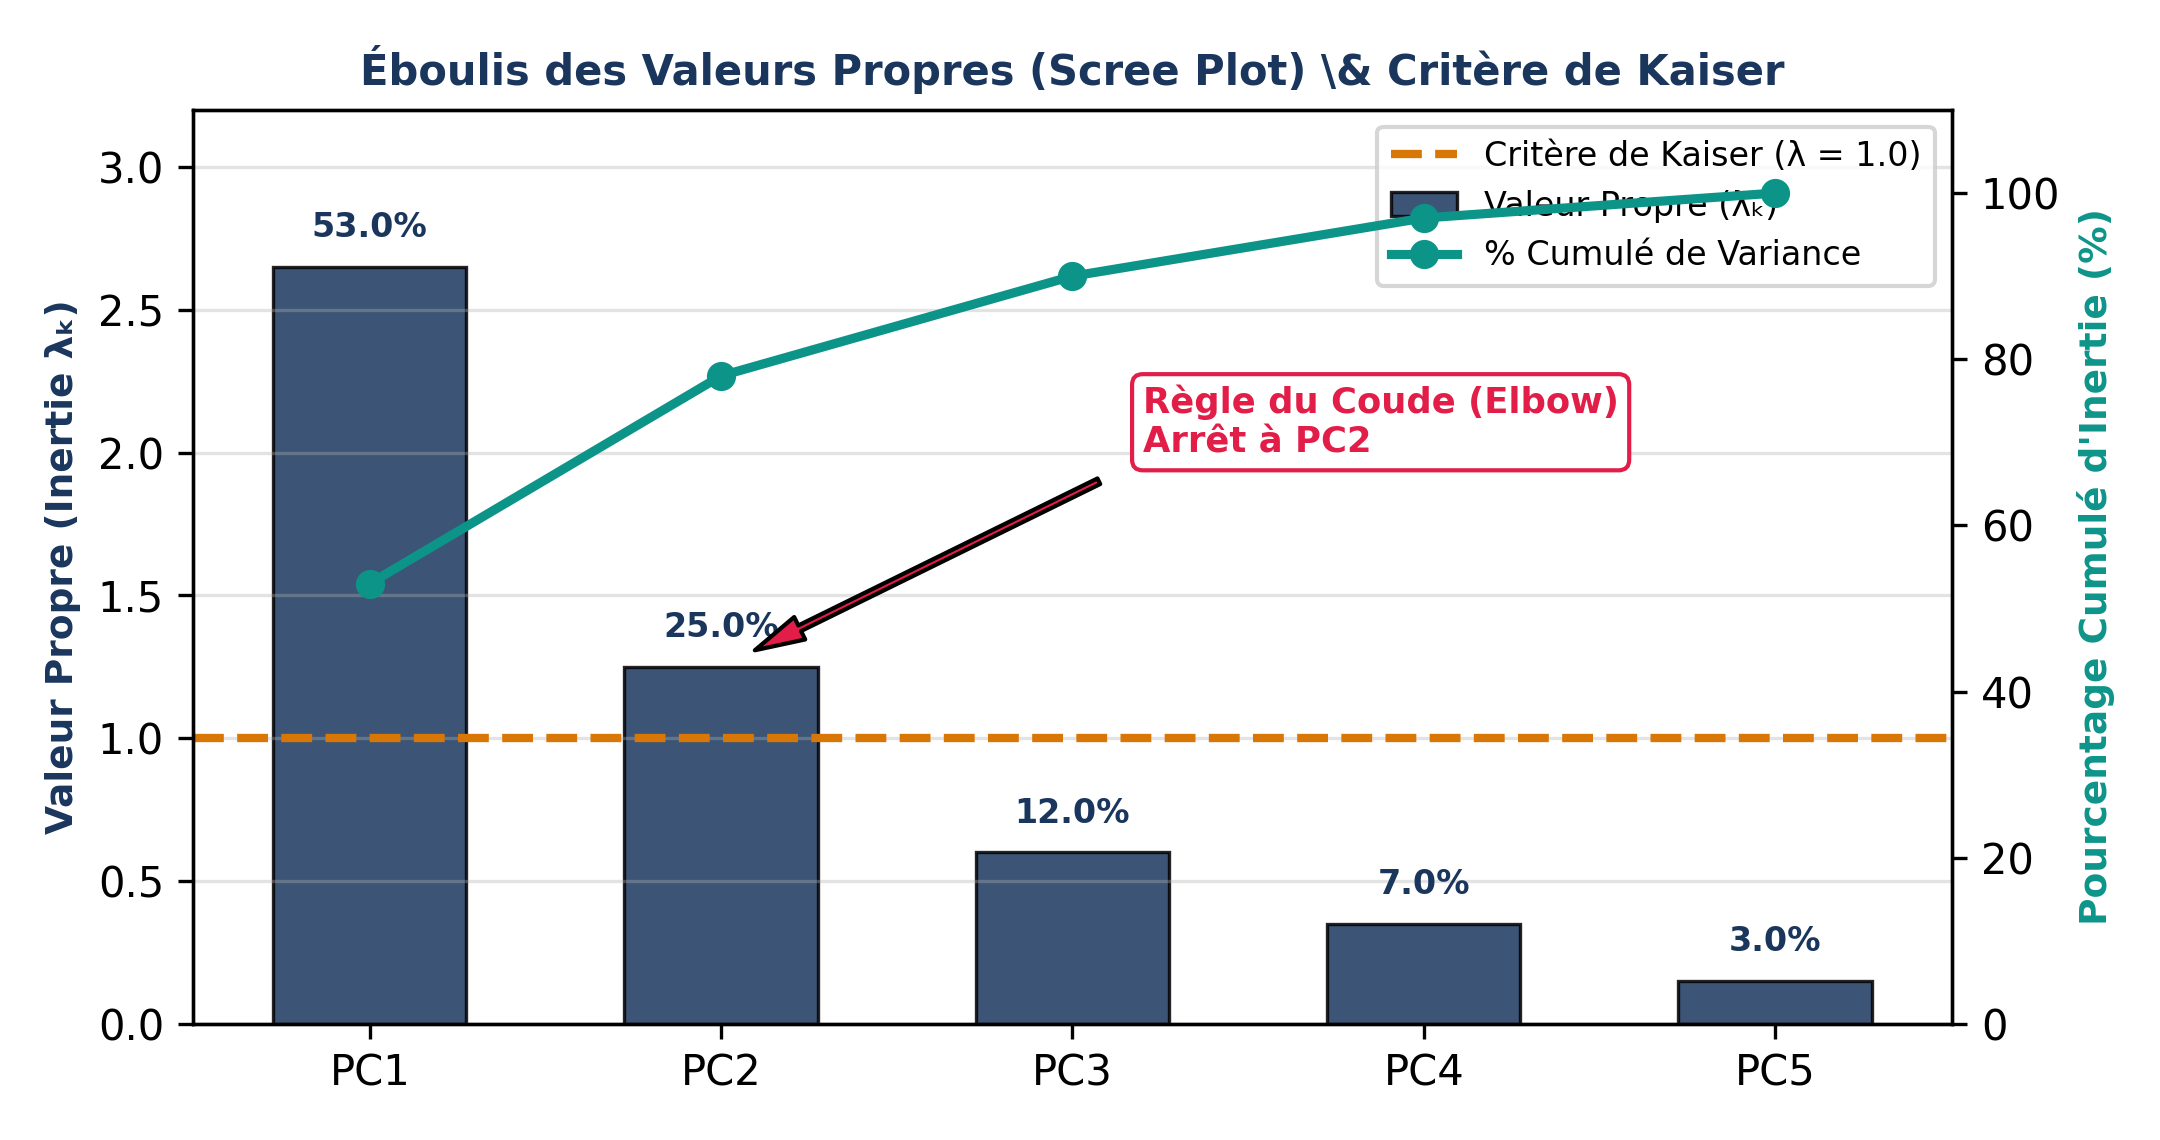
\includegraphics[height=0.55\textheight]{../figures/fig05_scree_plot_kaiser.png}
  \end{center}
  \vspace{-1mm}
  \begin{takeawaybox}{Décision Visuelle Immédiate}
    \scriptsize
    Les deux premières barres dépassent nettement la ligne pointillée de Kaiser ($\lambda = 1$). Le coude d'inflexion s'amorce à PC2. On retient le plan 2D (PC1 - PC2) sans hésitation.
  \end{takeawaybox}
\end{frame}

% ========================================================
\section{L'Espace des Variables : Le Cercle des Corrélations}
% ========================================================

% --- Diapositive 23 : Notion 14 : Coordonnees Variables ---
\begin{frame}{Notion 14 : Les Coordonnées des Variables sur les Axes (Loadings)}
  \begin{conceptbox}{Formule Mathématique des Coordonnées Factorielles}
    \footnotesize
    La coordonnée de la variable biologique $j$ sur l'axe principal $k$ est rigoureusement égale à son **coefficient de corrélation linéaire** avec cette composante :
    \begin{equation*}
      F_{jk} = \text{cor}(X_j, \text{PC}_k) = v_{jk} \sqrt{\lambda_k} \quad \text{avec } -1 \le F_{jk} \le +1
    \end{equation*}
  \end{conceptbox}
  \vspace{1mm}
  \begin{biobox}{Interprétation Directe pour le Biologiste}
    \footnotesize
    \begin{itemize}
      \item Si $F_{j1} = +0.92$ (cas de l'IL-6 sur PC1) : la cytokine est extraordinairement corrélée positivement à l'axe PC1.
      \item Si $F_{j1} = -0.80$ (cas de la Catalase sur PC1) : l'enzyme antioxydante est fortement corrélée négativement à PC1.
      \item $\implies$ Les coordonnées indiquent immédiatement le sens et l'intensité de liaison entre la molécule et l'axe.
    \end{itemize}
  \end{biobox}
\end{frame}

% --- Diapositive 24 : Notion 15 : Cercle Correlations ---
\begin{frame}{Notion 15 : Le Cercle des Corrélations de Rayon $R = 1$}
  \begin{conceptbox}{Construction Géométrique du Disque Unité}
    \footnotesize
    Puisqu'un coefficient de corrélation ne peut jamais dépasser $+1$ ni être inférieur à $-1$ :
    \begin{equation*}
      [r(X_j, \text{PC1})]^2 + [r(X_j, \text{PC2})]^2 \le 1 \implies \text{Toutes les variables sont contenues dans un cercle de rayon } 1
    \end{equation*}
  \end{conceptbox}
  \vspace{1mm}
  \begin{biobox}{Signification de la Longueur du Vecteur Variable}
    \footnotesize
    \begin{itemize}
      \item La flèche part de l'origine $(0,0)$ et se termine aux coordonnées $(F_{j1}, F_{j2})$.
      \item \textbf{Flèche proche de la circonférence ($r \to 1$) :} La variable est parfaitement expliquée et modélisée par le plan 1-2.
      \item \textbf{Flèche courte proche du centre $(0,0)$ :} La variable est mal représentée sur ce plan (son information est sur PC3 ou PC4).
    \end{itemize}
  \end{biobox}
\end{frame}

% --- Diapositive 25 : Notion 16 : Cos2 ---
\begin{frame}{Notion 16 : Qualité de Représentation d'une Variable : Le $\cos^2$}
  \begin{conceptbox}{Formule Mathématique du $\cos^2$}
    \footnotesize
    La proportion de variance de la variable $X_j$ captée par l'axe $k$ correspond au carré de sa coordonnée :
    \begin{equation*}
      \cos^2(X_j, \text{PC}_k) = [r(X_j, \text{PC}_k)]^2 = F_{jk}^2, \qquad \cos^2_{1+2} = \cos^2(X_j, \text{PC1}) + \cos^2(X_j, \text{PC2})
    \end{equation*}
  \end{conceptbox}
  \vspace{1mm}
  \begin{biobox}{Calcul Numérique Pas-à-Pas (Données TD 05)}
    \footnotesize
    \begin{itemize}
      \item \textbf{MDA ($F_1 = +0.88, F_2 = -0.20$) :} $\cos^2(\text{PC1}) = 0.88^2 = \mathbf{0.774}$, $\cos^2(\text{PC2}) = (-0.20)^2 = \mathbf{0.040}$.
      \item \textbf{Qualité globale sur le plan :} $\cos^2_{1+2} = 0.774 + 0.040 = \mathbf{0.814}$ (soit $81.4\%$ de sa variance expliquée).
      \item \textbf{Règle de validation :} Si $\cos^2_{1+2} \ge 0.60$, la variable est jugée très fidèlement représentée et son interprétation est solide.
    \end{itemize}
  \end{biobox}
\end{frame}

% --- Diapositive 26 : Notion 17 : Regle Angle Aigu ---
\begin{frame}{Notion 17 : Règle de Lecture 1 : Angle Aigu ($< 90^\circ$, Corrélation Positive)}
  \begin{conceptbox}{Signification Géométrique : Flèches Pointant dans la Même Direction}
    \footnotesize
    Le cosinus de l'angle $\theta$ entre deux vecteurs variables approxime leur coefficient de corrélation mutuel :
    \begin{equation*}
      \cos(\theta) \approx r(X_j, X_l) \implies \text{Angle aigu } (\theta < 90^\circ) \iff r(X_j, X_l) > 0
    \end{equation*}
  \end{conceptbox}
  \vspace{1mm}
  \begin{biobox}{Interprétation Biologique Concrète}
    \footnotesize
    \textbf{Faisceau IL-6, TNF-$\alpha$ et MDA :}
    \begin{itemize}
      \item Les flèches de l'IL-6 ($+0.92$) et du MDA ($+0.88$) forment un angle très fermé ($\theta \approx 15^\circ$).
      \item $\implies$ L'élévation de la cytokine pro-inflammatoire s'accompagne systématiquement d'une flambée de peroxydation lipidique membranaire chez l'animal malade.
      \item Deux variables très proches sont \textbf{redondantes} dans le panel diagnostique.
    \end{itemize}
  \end{biobox}
\end{frame}

% --- Diapositive 27 : Notion 18 : Regle Angle Droit ---
\begin{frame}{Notion 18 : Règle de Lecture 2 : Angle Droit ($\approx 90^\circ$, Indépendance)}
  \begin{conceptbox}{Signification Géométrique : Vecteurs Orthogonaux}
    \footnotesize
    Deux flèches formant un angle proche de $90^\circ$ ont un cosinus nul :
    \begin{equation*}
      \cos(90^\circ) = 0 \iff r(X_j, X_l) \approx 0 \quad \text{(Absence totale de corrélation linéaire)}
    \end{equation*}
  \end{conceptbox}
  \vspace{1mm}
  \begin{biobox}{Interprétation Biologique Concrète}
    \footnotesize
    \textbf{SOD ($F_1 = -0.10, F_2 = +0.85$) vs MDA ($F_1 = +0.88, F_2 = -0.20$) :}
    \begin{itemize}
      \item Les deux flèches sont quasiment perpendiculaires ($\theta \approx 95^\circ$).
      \item $\implies$ L'activité enzymatique de la superoxyde dismutase (SOD) varie de manière totalement indépendante de la peroxydation du MDA.
      \item Ces deux molécules explorent deux facettes physiologiques distinctes et non redondantes !
    \end{itemize}
  \end{biobox}
\end{frame}

% --- Diapositive 28 : Notion 19 : Regle Angle Plat ---
\begin{frame}{Notion 19 : Règle de Lecture 3 : Angle Plat ($\approx 180^\circ$, Antagonisme)}
  \begin{conceptbox}{Signification Géométrique : Flèches Diamétralement Opposées}
    \footnotesize
    Deux flèches pointant dans des directions opposées forment un angle proche de $180^\circ$ :
    \begin{equation*}
      \cos(180^\circ) = -1 \iff r(X_j, X_l) < 0 \quad \text{(Forte corrélation négative / Anti-corrélation)}
    \end{equation*}
  \end{conceptbox}
  \vspace{1mm}
  \begin{biobox}{Interprétation Biologique Concrète}
    \footnotesize
    \textbf{Catalase ($F_1 = -0.80$) vs MDA ($F_1 = +0.88$) :}
    \begin{itemize}
      \item Les deux flèches pointent à l'opposé le long de l'axe horizontal PC1.
      \item $\implies$ Quand la peroxydation lipidique (MDA) s'effondre chez les témoins sains, la défense antioxydante hépatique par la Catalase est maximale.
      \item À l'inverse, l'oxydation sévère chez les souris malades s'accompagne d'un épuisement enzymatique en Catalase.
    \end{itemize}
  \end{biobox}
\end{frame}

% --- Diapositive 29 : Notion 20 : Contribution Variables ---
\begin{frame}{Notion 20 : Contribution d'une Variable à l'Axe ($\text{CTR}$)}
  \begin{conceptbox}{Formule Mathématique de la Contribution}
    \footnotesize
    Pourcentage de l'inertie de l'axe $\text{PC}_k$ apporté par la variable $X_j$ :
    \begin{equation*}
      \text{CTR}_{jk} = \frac{F_{jk}^2}{\lambda_k} \times 100 \quad \text{avec } \sum_{j=1}^p \text{CTR}_{jk} = 100\%
    \end{equation*}
    \textbf{Seuil de significativité théorique :} Une variable contribue significativement à l'axe si sa contribution dépasse la moyenne équitable : $\text{CTR} > \frac{100\%}{p} = \frac{100\%}{5} = \mathbf{20.0\%}$.
  \end{conceptbox}
  \vspace{1mm}
  \begin{biobox}{Dénomination Biologique Objective de l'Axe PC1}
    \footnotesize
    \begin{itemize}
      \item Contribution de l'IL-6 à PC1 : $\text{CTR} = \frac{0.92^2}{2.65} \times 100 = \frac{0.8464}{2.65} \times 100 = \mathbf{31.9\%} \gg 20\%$.
      \item Contribution du MDA à PC1 : $\text{CTR} = \frac{0.88^2}{2.65} \times 100 = \frac{0.7744}{2.65} \times 100 = \mathbf{29.2\%} \gg 20\%$.
      \item $\implies$ L'axe PC1 est formellement baptisé : **« Axe du Stress Oxydant \& de l'Inflammation Aiguë »**.
    \end{itemize}
  \end{biobox}
\end{frame}

% ========================================================
\section{L'Espace des Individus : Le Plan Factoriel des Scores (Score Plot)}
% ========================================================

% --- Diapositive 30 : Notion 21 : Calcul des Scores ---
\begin{frame}{Notion 21 : Coordonnées des Échantillons : Les Scores Factoriels}
  \begin{conceptbox}{Formule Mathématique du Score Individuel}
    \footnotesize
    Chaque individu biologique (souris ou patient $i$) reçoit une nouvelle coordonnée $S_{ik}$ sur l'axe $\text{PC}_k$ par combinaison linéaire de ses $Z$-scores :
    \begin{equation*}
      S_{ik} = \sum_{j=1}^p Z_{ij} v_{jk} = Z_{i1} v_{1k} + Z_{i2} v_{2k} + \dots + Z_{ip} v_{pk}
    \end{equation*}
    Cette valeur sans dimension $S_{ik}$ est le **Score Factoriel**.
  \end{conceptbox}
  \vspace{1mm}
  \begin{biobox}{Sens Clinique des Scores}
    \footnotesize
    \begin{itemize}
      \item Un patient avec un score $S_{i1} = +3.2$ se situe très loin à droite sur l'axe du stress oxydant.
      \item Le tableau initial $n \times p$ (ex: $40 \times 7$) est désormais réduit à un tableau léger $n \times 2$ ($40 \times 2$ scores : PC1 et PC2).
      \item On peut représenter l'ensemble des 40 malades sur un plan cartésien 2D classique !
    \end{itemize}
  \end{biobox}
\end{frame}

% --- Diapositive 31 : Notion 22 : Proprietes Scores ---
\begin{frame}{Notion 22 : Propriétés Statistiques Fondamentales des Scores}
  \begin{conceptbox}{Centrage \& Variance des Composantes Principales}
    \footnotesize
    \begin{itemize}
      \item \textbf{Moyenne Nulle :} $\mathbb{E}(\text{PC}_k) = \frac{1}{n} \sum_{i=1}^n S_{ik} = 0$ \quad $\implies$ Le centre $(0,0)$ est le « profil moyen ».
      \item \textbf{Variance Égale à la Valeur Propre :} $\text{Var}(\text{PC}_k) = \frac{1}{n} \sum_{i=1}^n S_{ik}^2 = \lambda_k$ \quad $\implies$ Dispersion égale à $\lambda_k$.
      \item \textbf{Orthogonalité Absolue :} $\text{cor}(\text{PC}_k, \text{PC}_l) = 0$ pour tout $k \neq l$.
    \end{itemize}
  \end{conceptbox}
  \vspace{1mm}
  \begin{takeawaybox}{Conséquence Visuelle}
    \footnotesize
    Le nuage des scores est toujours plus étiré horizontalement le long de PC1 que verticalement le long de PC2 car $\lambda_1 > \lambda_2$.
  \end{takeawaybox}
\end{frame}

% --- Diapositive 32 : Notion 23 : Interprétation Conjointe ---
\begin{frame}{Notion 23 : L'Interprétation Conjointe (Biplot Conceptuel)}
  \begin{conceptbox}{Règle de Superposition des Deux Espaces}
    \footnotesize
    L'espace des variables (cercle) et l'espace des individus (score plot) s'interprètent en miroir direct :
  \end{conceptbox}
  \vspace{1mm}
  \begin{biobox}{La Clé de Lecture Physiopathologique}
    \footnotesize
    \begin{itemize}
      \item Un patient projeté dans la région où pointent les flèches IL-6 et MDA présente des taux sériques anormalement élevés de ces deux marqueurs.
      \item Un patient projeté à l'opposé exact de ces flèches possède des taux bas d'IL-6 et de MDA, mais des taux élevés de Catalase.
      \item Les individus proches du centre $(0,0)$ possèdent un profil standard sans anomalie biologique saillante.
    \end{itemize}
  \end{biobox}
\end{frame}

% --- Diapositive 33 : Visualisation Biplot / Score Plot ---
\begin{frame}{Visualisation Graphique : Cercle des Corrélations \& Plan des Patients}
  \begin{center}
    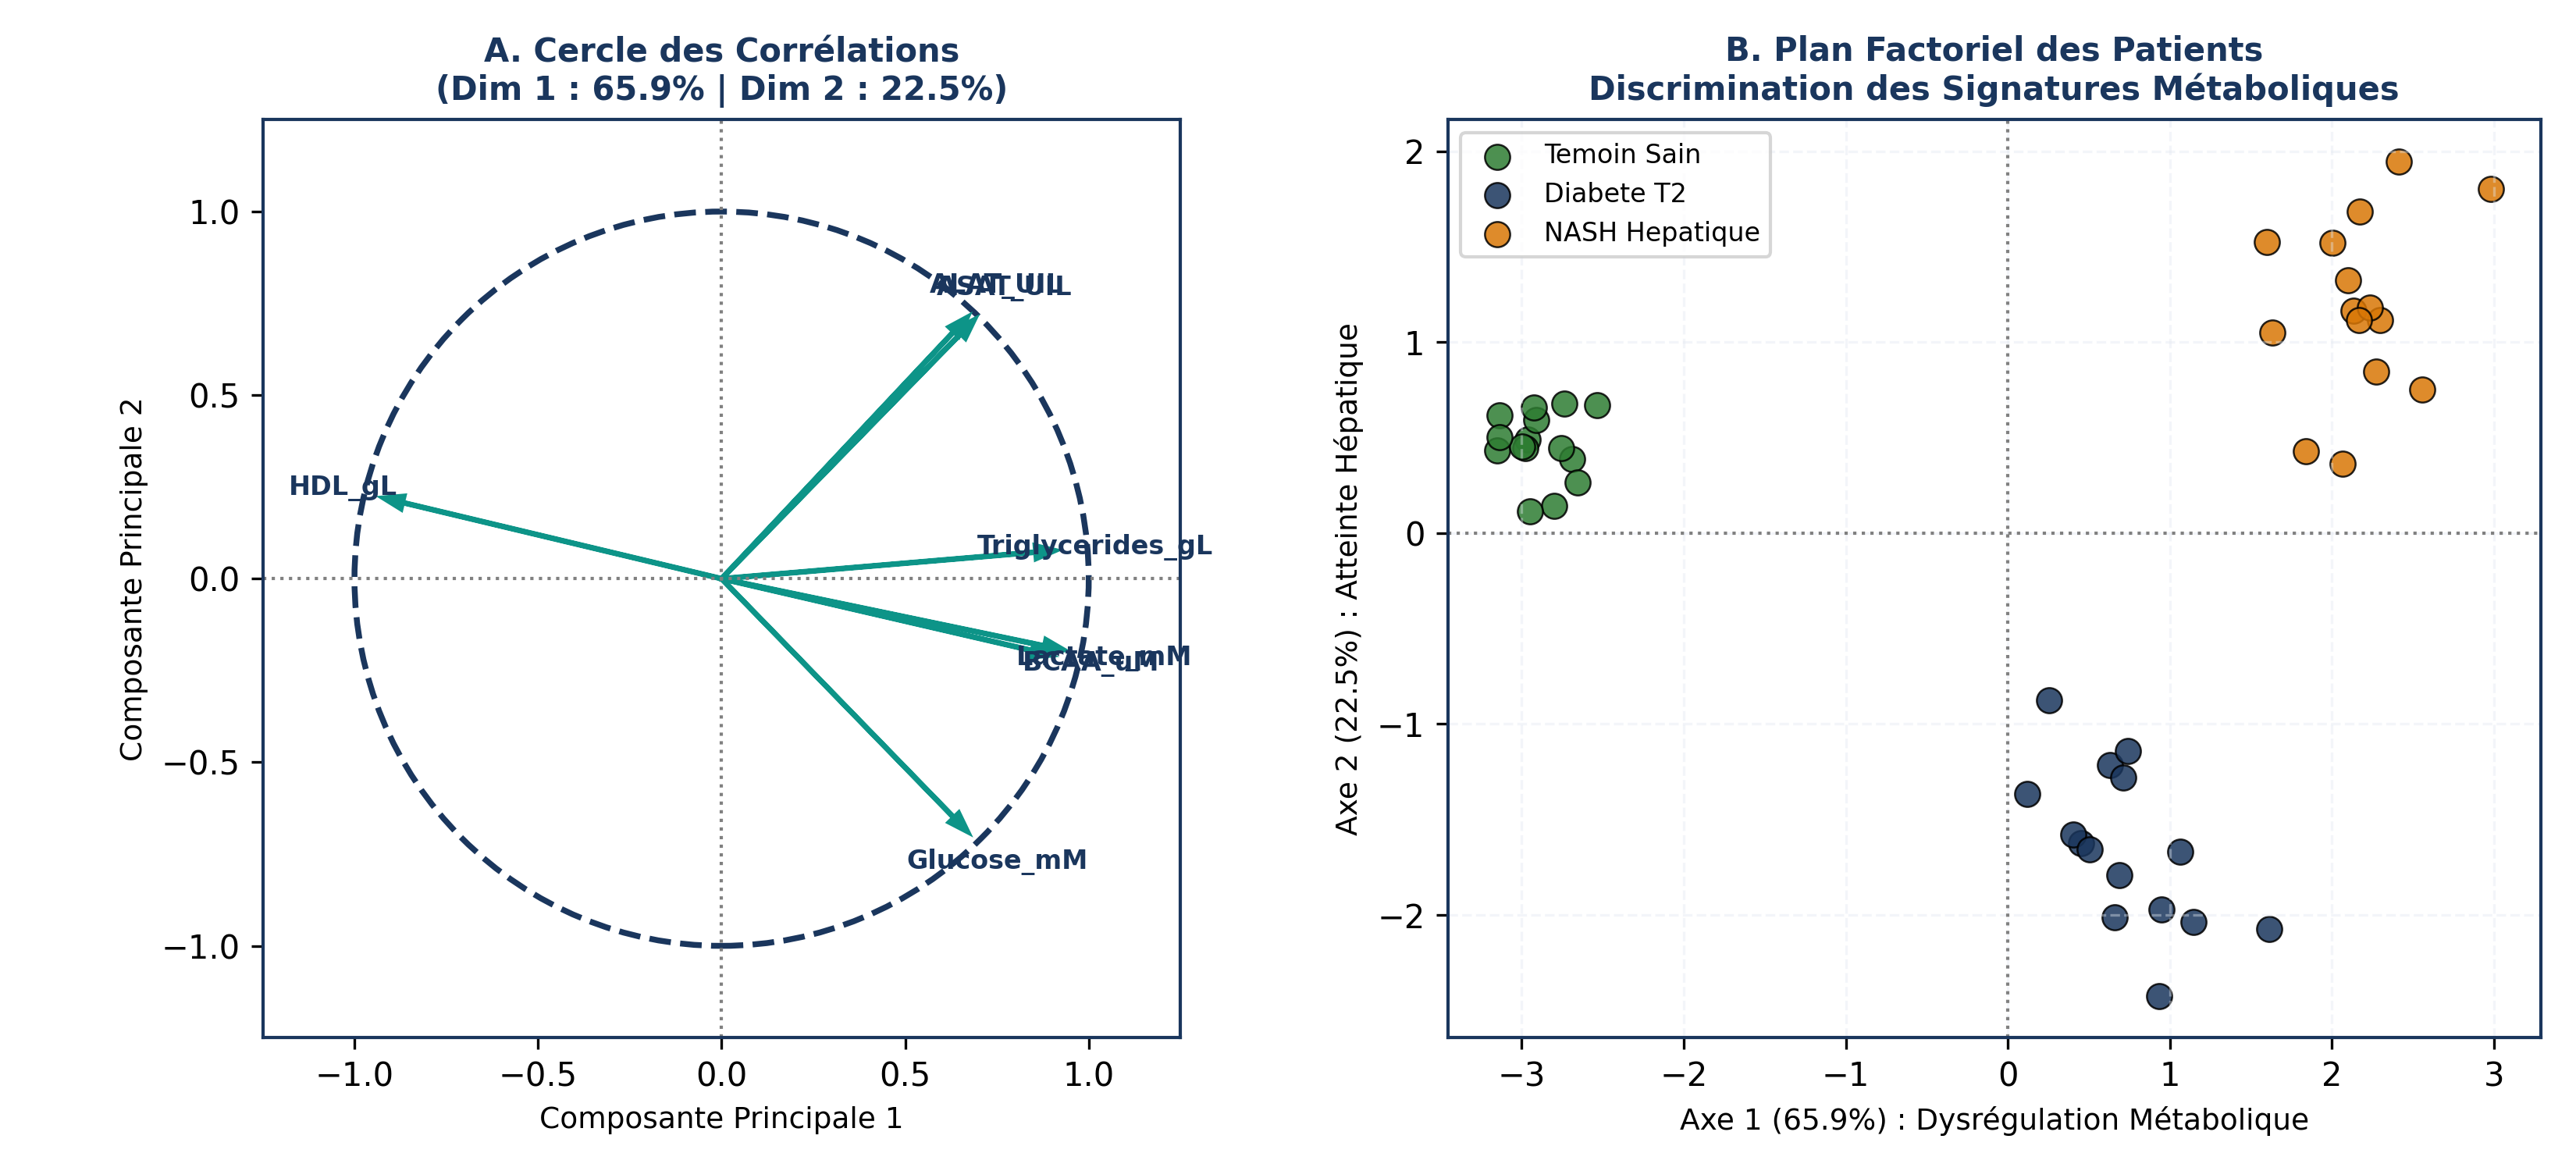
\includegraphics[height=0.55\textheight]{../figures/fig05_pca_correlation_and_scores.png}
  \end{center}
  \vspace{-1mm}
  \begin{takeawaybox}{Séparation Métabolique Clinique Nette}
    \scriptsize
    À gauche : Cercle des variables identifiant les clusters métaboliques. À droite : Plan des patients séparant parfaitement les Témoins sains (vert), les Diabétiques (bleu sur l'Axe 1) et les Stéatohépatites NASH (orange sur l'Axe 2).
  \end{takeawaybox}
\end{frame}

% --- Diapositive 34 : Notion 24 : Non Supervise ---
\begin{frame}{Notion 24 : La Nature Non Supervisée de l'ACP}
  \begin{conceptbox}{Définition Statistique : Aucune Connaissance Préalable des Classes}
    \footnotesize
    L'ACP est un algorithme \textbf{strictement non supervisé} :
    \begin{itemize}
      \item La matrice de calcul $Z$ ne contient que les concentrations biochimiques continues ($X_j$).
      \item Le diagnostic clinique ou le groupe de traitement (Témoin, Diabétique, NASH) n'est \textbf{jamais fourni au modèle}.
    \end{itemize}
  \end{conceptbox}
  \vspace{1mm}
  \begin{biobox}{Pourquoi le Regroupement Spontané a-t-il une Valeur Inestimable ?}
    \footnotesize
    \begin{itemize}
      \item Lorsque les individus d'un même groupe se rassemblent spontanément en amas distincts sur le graphique, c'est la démonstration rigoureuse que **l'empreinte biologique globale porte la signature intrinsèque de la pathologie**.
      \item Cela valide la pertinence du panel omique sans biais de sélection artificiel.
    \end{itemize}
  \end{biobox}
\end{frame}

% --- Diapositive 35 : Notion 25 : Individus Supplementaires ---
\begin{frame}{Notion 25 : Projection d'Individus \& Variables Supplémentaires}
  \begin{conceptbox}{Principe des Éléments Illustratifs (Passifs)}
    \footnotesize
    On peut projeter de nouvelles observations sans recalculer ni déformer les axes de référence :
    \begin{equation*}
      S_{\text{nouveau}, k} = \sum_{j=1}^p \left(\frac{X_{\text{nouveau}, j} - \bar{X}_j}{s_j}\right) v_{jk}
    \end{equation*}
  \end{conceptbox}
  \vspace{1mm}
  \begin{biobox}{Application au Diagnostic d'un Patient Inconnu}
    \footnotesize
    \textbf{Cas d'un nouveau patient admis aux urgences :}
    \begin{itemize}
      \item On dose ses 7 biomarqueurs plasmatiques. On calcule ses coordonnées : $\text{PC1} = +2.40, \, \text{PC2} = +1.85$.
      \item En reportant ce point sur le plan de référence, il tombe en plein cœur du cluster « Atteinte Hépatique NASH ».
      \item L'ACP oriente immédiatement le clinicien vers une biopsie hépatique ciblée !
    \end{itemize}
  \end{biobox}
\end{frame}

% ========================================================
\section{Pièges Méthodologiques, Sélection de Biomarqueurs \& Synthèse}
% ========================================================

% --- Diapositive 36 : Notion 26 : Piege Cos2 Faible ---
\begin{frame}{Notion 26 : Piège 1 : Les Variables Mal Représentées ($\cos^2$ Faible)}
  \begin{warnbox}{L'Illusion d'Optique des Variables Proches du Centre}
    \footnotesize
    \begin{itemize}
      \item Si une flèche est courte et reste proche de l'origine (ex: longueur $r < 0.40 \implies \cos^2 < 0.16$), la variable est située hors du plan 1-2.
      \item \textbf{Erreur grave fréquente :} Déduire que cette molécule n'a aucun rôle ou qu'elle est indépendante des autres.
      \item \textbf{Réalité :} Son information s'exprime sur les axes suivants (PC3 ou PC4). Interpréter sa proximité sur le plan 1-2 est un contresens géométrique !
    \end{itemize}
  \end{warnbox}
  \vspace{1mm}
  \begin{takeawaybox}{Règle de Bonne Pratique}
    \footnotesize
    Ne jamais interpréter la position d'une variable dont la qualité de représentation globale $\cos^2_{1+2}$ est inférieure à $0.50$ (ou examiner son cercle sur le plan 1-3).
  \end{takeawaybox}
\end{frame}

% --- Diapositive 37 : Notion 27 : Piege Effet Taille ---
\begin{frame}{Notion 27 : Piège 2 : L'Effet Taille (Size Effect) en Morphométrie}
  \begin{warnbox}{Quand l'Axe 1 N'est qu'un Réflecteur de Corpulence}
    \footnotesize
    En biologie animale et pharmacologie :
    \begin{itemize}
      \item Si toutes les variables sont morphométriques ou de volumétrie tissulaire (poids foie, poids rate, adiposité, longueur du tibia), toutes les corrélations $r_{jk}$ sont positives.
      \item L'axe PC1 capte alors un pur **« Effet de Taille »** général ($\lambda_1 > 80\%$).
      \item Les animaux se classent simplement du plus petit au plus gros sur PC1.
    \end{itemize}
  \end{warnbox}
  \vspace{1mm}
  \begin{takeawaybox}{Où se Cache l'Information Biologique Fine ?}
    \footnotesize
    Dans ce cas précis, la véritable information de forme ou de dysfonction d'organe spécifique réside sur l'\textbf{Axe PC2} (qui oppose par exemple le volume adipeux à la masse musculaire). Le chercheur averti doit regarder l'axe secondaire !
  \end{takeawaybox}
\end{frame}

% --- Diapositive 38 : Notion 28 : Selection Biomarqueurs ---
\begin{frame}{Notion 28 : Sélection de Biomarqueurs \& Élimination de la Redondance}
  \begin{conceptbox}{Conception d'une Trousse de Diagnostic Rapide (Point-of-Care)}
    \footnotesize
    Doser 10 biomarqueurs en routine hospitalière est coûteux et redondant. L'ACP permet d'extraire le panel minimal d'information maximale :
  \end{conceptbox}
  \vspace{1mm}
  \begin{biobox}{Application Stratégique au Panel du TD 05}
    \footnotesize
    \begin{enumerate}
      \item \textbf{Axe PC1 (Inflammation / Stress oxydant) :} L'IL-6 ($F_1 = 0.92, \cos^2 = 0.85$) et le TNF-$\alpha$ ($F_1 = 0.85, \cos^2 = 0.72$) sont redondants. On conserve uniquement **l'IL-6**, molécule la mieux corrélée à l'axe.
      \item \textbf{Axe PC2 (Défense antioxydante spécifique) :} La **SOD** ($F_2 = 0.85, \cos^2 = 0.72$) capture orthogonalement l'axe 2.
      \item \textbf{Bilan analytique :} Deux biomarqueurs bien choisis (IL-6 + SOD) suffisent à capturer l'ensemble de la cartographie pathologique avec une économie réactive de $60\%$ !
    \end{enumerate}
  \end{biobox}
\end{frame}

% --- Diapositive 39 : Synthese Methodologique ---
\begin{frame}{Synthèse : L'Algorithme Décisionnel de l'ACP pour le Biochimiste}
  \begin{conceptbox}{Phase 1 : Préparation \& Validation Algébrique}
    \footnotesize
    \begin{itemize}
      \item Centrer et réduire la matrice : $Z_{ij} = (X_{ij} - \bar{X}_j)/s_j \longrightarrow$ Calculer la matrice des corrélations $R$.
      \item Extraire les valeurs propres $\lambda_k$ $\longrightarrow$ Vérifier $\sum \lambda_k = p$.
      \item Choisir le nombre d'axes via Kaiser ($\lambda \ge 1$) et l'éboulis (scree plot) pour atteindre $> 70\text{--}80\%$ d'inertie.
    \end{itemize}
  \end{conceptbox}
  \vspace{1mm}
  \begin{biobox}{Phase 2 : Interprétation Biologique Conjointe (Biplot)}
    \footnotesize
    \begin{itemize}
      \item \textbf{Cercle des variables :} Vérifier les $\cos^2$, interpréter les angles (aigus = co-régulation, droits = indépendance, plats = antagonisme). Nommer les axes avec les $\text{CTR}$.
      \item \textbf{Plan des individus :} Repérer les clusters spontanés, identifier les phénotypes atypiques, projeter les inconnus.
    \end{itemize}
  \end{biobox}
\end{frame}

% --- Diapositive 40 : Conclusion & Ouverture ---
\begin{frame}[plain]
  \begin{center}
    \vspace{1.5cm}
    {\Huge\color{BioNavy}\textbf{Fin du Chapitre V}}\\[0.6cm]
    {\large\color{BioTeal}\textbf{Félicitations ! Vous maîtrisez la réduction factorielle et l'ACP normée.}}\\[1.0cm]
    {\normalsize\textbf{Prochaine étape : Comment regrouper automatiquement les profils d'individus en classes homogènes ?}}\\[0.3cm]
    {\large\textbf{Chapitre VI : Classification Ascendante Hiérarchique (CAH) \& Dendrogrammes}}\\[1.2cm]
    \textbf{Dr. Sarra BENMOUMOU-HOSNI (Ph.D.)}\\
    \small Faculté des Sciences --- Département de Biologie\\
    \textbf{Université M'Hamed Bougara de Boumerdès (UMBB)}
  \end{center}
\end{frame}

\end{document}
